% Supplementary material. This file is intended to be included after
% \appendix in the final paper source.

\section{Additional Experimental Details}

Policy generation and revision use supply seed 42. Frozen-policy replay uses
seeds $\{10,42,98,197,666\}$, where seed 42 is the experienced trajectory and
the other four sequences are held out from policy generation.

\section{Objective Outcome Intervals}

\begin{table*}[t]
    \centering
    \small
    \caption{Role-balanced revised-policy performance with 95\% matched
    experiment-cluster bootstrap intervals. Values average MR2--MR3 after
    averaging the five fixed evaluation seeds within each experiment.}
    \label{tab:objective-performance-ci}
    % Generated by src/objective_outcomes/analyze_objective_outcomes.py
\begin{tabular}{llrr}
    \toprule
    Model & Feedback & WACScore (95\% CI) & Mortality (95\% CI) \\
    \midrule
    Gemini 3.5 Flash & OF & 86.47 [84.81, 88.07] & 25.75 [23.26, 28.49] \\
     & OPF & 87.05 [85.00, 89.12] & 25.08 [21.70, 28.31] \\
    \addlinespace
    Claude Sonnet 5 & OF & 86.17 [84.25, 88.14] & 25.00 [22.48, 27.61] \\
     & OPF & 84.05 [81.64, 86.45] & 28.67 [25.06, 32.32] \\
    \addlinespace
    GPT-5.4 & OF & 84.27 [81.59, 86.82] & 27.58 [23.95, 31.23] \\
     & OPF & 81.72 [78.99, 84.22] & 31.08 [27.75, 34.65] \\
    \addlinespace
    DeepSeek V4 Flash & OF & 69.04 [64.66, 73.30] & 45.83 [40.48, 51.35] \\
     & OPF & 67.84 [64.46, 71.17] & 46.58 [42.53, 50.74] \\
    \addlinespace
    GPT-5.4 Nano & OF & 50.95 [46.40, 55.45] & 66.42 [60.99, 72.06] \\
     & OPF & 65.35 [62.16, 68.39] & 48.83 [44.92, 52.82] \\
    \bottomrule
\end{tabular}

\end{table*}

\section{Additional Adaptation Results}
\label{app:adaptation-details}

The main paper reports the aggregate MR1--MR3 trajectories. Here we
separate those trajectories by model backend and report the adjacent-round
changes. Estimates use the same five fixed evaluation supply seeds and
matched experiment-cluster bootstrap procedure as the main analysis.

\begin{figure*}[t]
    \centering
    \includegraphics[width=\textwidth]{../compare_result/adaptation_dynamics/adaptation_by_model.png}
    \caption{Model-level WACScore and mortality trajectories under Outcome
    Feedback (OF) and Outcome-and-Policy Feedback (OPF). Shaded regions
    denote 95\% matched experiment-cluster bootstrap intervals after
    averaging the five evaluation seeds within each experiment.}
    \label{fig:adaptation-by-model}
\end{figure*}

Figure~\ref{fig:adaptation-by-model} shows that the aggregate OPF trend is
not a uniform shift shared by every backend. Claude improves primarily
after the first revision, while GPT-5.4 continues to benefit under OPF.
Gemini remains comparatively stable at a high performance level.
DeepSeek exhibits weaker and less consistent revision, and GPT-5.4 Nano
shows the clearest feedback-dependent divergence: its OF trajectory
regresses while its OPF trajectory improves. These patterns suggest that
policy transparency is most useful when a backend can translate observed
opponent logic into an executable revision without destabilizing an
already effective policy.

\begin{figure*}[t]
    \centering
    \includegraphics[width=0.9\textwidth]{../compare_result/adaptation_dynamics/adaptation_changes.png}
    \caption{Paired adjacent-round and full-horizon changes in WACScore
    and mortality. Error bars show 95\% matched experiment-cluster
    bootstrap intervals.}
    \label{fig:adaptation-changes}
\end{figure*}

The paired changes in Figure~\ref{fig:adaptation-changes} reinforce the
trajectory-level observation. Both conditions benefit from the first
revision, but only OPF shows a clear positive WACScore change from MR2 to
MR3. Mortality changes are noisier, indicating that longer average
survival and avoidance of catastrophic failure capture related but
distinct properties of a revised policy.

\begin{figure*}[t]
    \centering
    \includegraphics[width=0.92\textwidth]{../compare_result/adaptation_dynamics/model_revision_effects.png}
    \caption{Model-level baseline-adjusted policy-transparency effects from
    MR1 to MR3. Points are OPF-minus-OF differences in changes; error bars
    are 95\% matched experiment-cluster bootstrap intervals. Positive
    values favor OPF for WACScore, whereas negative values favor OPF for
    mortality.}
    \label{fig:model-revision-effects}
\end{figure*}

Only GPT-5.4 Nano has intervals excluding zero for both outcomes in
Figure~\ref{fig:model-revision-effects}. The remaining model-level effects
are exploratory and should not be interpreted as evidence of no effect.

\section{Additional Policy-Convergence Diagnostics}
\label{app:policy-convergence-details}

\begin{figure}[t]
    \centering
    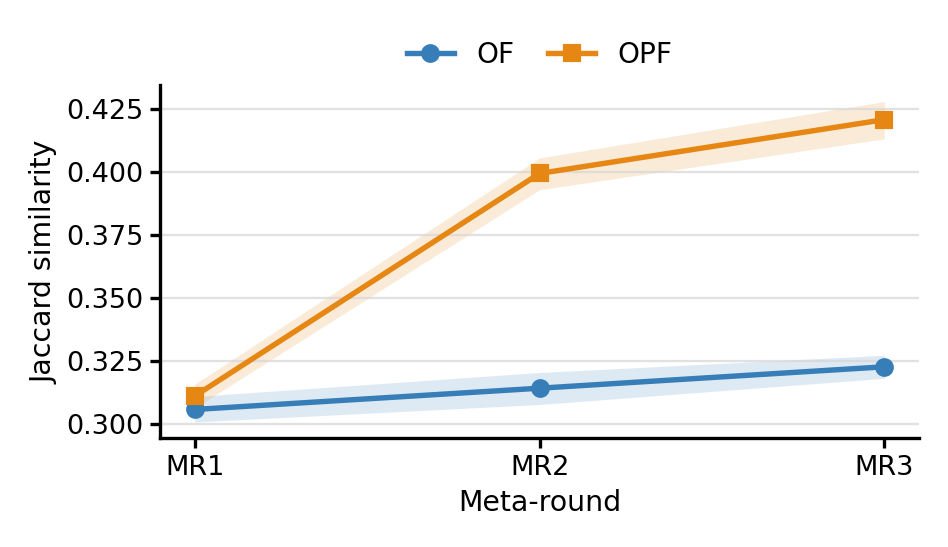
\includegraphics[width=0.90\linewidth]{policy_structure_similarity.png}
    \caption{Structural policy convergence measured by pairwise Jaccard
    similarity over normalized AST node-type 3-grams. Higher values indicate
    more similar program structure; bands are 95\% matched
    experiment-cluster bootstrap intervals.}
    \label{fig:policy-structure-similarity}
\end{figure}

\begin{figure*}[t]
    \centering
    \includegraphics[width=0.92\textwidth]{../compare_result/adaptation_dynamics/performance_dispersion.png}
    \caption{Descriptive dispersion across the five role-balanced model
    means. Bands are matched experiment-cluster bootstrap intervals.}
    \label{fig:performance-dispersion}
\end{figure*}

The outcome dispersion in Figure~\ref{fig:performance-dispersion} moves in
the same direction as the controlled policy probes: dispersion rises over
meta-rounds under OF and falls by MR3 under OPF. Because the baseline-adjusted
MR1-to-MR3 interval approaches zero for WACScore and includes zero for
mortality, we use this result only as descriptive corroboration of the
behavioral convergence analysis.

\section{Additional Policy Diagnostics}
\label{app:secondary-diagnostics}

Counterfactual planning and risk response isolate narrower aspects of policy
behavior than the primary simulator-grounded outcomes. They are diagnostic
rather than an exhaustive definition of strategic competence and do not
replace WACScore or mortality. We additionally give the model-level
disaggregation of FOSG, whose aggregate result is part of the main evidence
for effective revision.

\subsection{Counterfactual Planning}

We use paired counterfactual rollouts at fixed checkpoints, comparing the
policy bid $a_\pi$ with a discrete set $\mathcal{A}$ of budget-scaled bids
under shared future supply sequences. Counterfactual Survival Regret (CSR)
measures the expected survival days lost relative to the best tested action:
\begin{equation}
    \mathrm{CSR}
    =
    \mathbb{E}_{s}\!\left[
        \max_{a\in\mathcal{A}}
        \mathbb{E}_{\omega}[R(s,a,\omega)]
        -
        \mathbb{E}_{\omega}[R(s,a_\pi,\omega)]
    \right],
\end{equation}
where $R(s,a,\omega)$ is remaining survival from state $s$ after action $a$
under rollout $\omega$. Lower CSR is better; its reference is the best tested
action rather than the global continuous optimum. CSR is conditional on the
policy reaching the evaluated checkpoint.

\subsection{Risk-Response}

We probe generated policies offline by holding the decision context fixed
while increasing health risk, drought risk, or both. Normalized Bid Adjustment
(NBA) measures the signed change in the policy's bid relative to available
budget $B$:
\begin{equation}
    \mathrm{NBA}
    =
    \mathbb{E}\!\left[
        \frac{b_{\mathrm{risk}}-b_{\mathrm{safe}}}{B}
    \right].
\end{equation}
We average NBA over the three risk manipulations and controlled background
states. Larger values indicate a stronger upward bid adjustment under risk;
NBA is descriptive and does not by itself imply better decision quality.

\subsection{Frozen-Opponent Revision}

Frozen-Opponent Survival Gain (FOSG) measures whether replacing only the
focal MR1 policy with its MR2 revision improves survival against unchanged
MR1 opponents under common seeds:
\begin{equation}
    \mathrm{FOSG}
    =
    \mathbb{E}_{a,i,s}\!\left[
        D_i\!\left(\pi_i^{(2)},\pi_{-i}^{(1)};s\right)
        -D_i\!\left(\pi_i^{(1)},\pi_{-i}^{(1)};s\right)
    \right],
\end{equation}
where $a$ indexes model-to-role permutations, $i$ is the focal agent, $s$
indexes replay supply sequences, and $D_i$ is the focal agent's survival
duration. Positive FOSG means that the revised policy improves survival with
opponents held fixed. FOSG measures effective revision rather than
responsiveness alone. Comparing it under OF and OPF tests whether
opponent-policy access improves revision, but does not establish that a model
formed an internal representation of its opponents.

\subsection{Model-Level Diagnostic Results}

\begin{table}[t]
    \centering
    \small
    \setlength{\tabcolsep}{3.2pt}
    \caption{Model-level policy diagnostics under OF and OPF. CSR and FOSG
    are measured in survival days; NBA is a percentage of available budget
    and has no monotonic better direction. FOSG uses paired MR1-to-MR2
    frozen-opponent replays.}
    \label{tab:capability-diagnostics}
    \begin{tabular}{llrrr}
        \toprule
        Model & Feedback & CSR $\downarrow$ & NBA (\%) & FOSG $\uparrow$ \\
        \midrule
        Gemini 3.5 Flash
            & OF  & 0.091 & 29.0 & 0.470 \\
            & OPF & 0.080 & 28.1 & 0.263 \\
            & Avg. & 0.086 & 28.6 & 0.367 \\
        \addlinespace
        Claude Sonnet 5
            & OF  & \textbf{0.037} & 16.3 & \textbf{1.022} \\
            & OPF & \textbf{0.030} & 18.5 & 0.912 \\
            & Avg. & \textbf{0.033} & 17.4 & \textbf{0.967} \\
        \addlinespace
        GPT-5.4
            & OF  & 0.054 & 22.4 & 0.587 \\
            & OPF & 0.096 & 23.1 & \textbf{0.918} \\
            & Avg. & 0.075 & 22.7 & 0.753 \\
        \addlinespace
        DeepSeek V4 Flash
            & OF  & 0.439 & 13.7 & 0.123 \\
            & OPF & 0.320 & 15.1 & 0.602 \\
            & Avg. & 0.379 & 14.4 & 0.363 \\
        \addlinespace
        GPT-5.4 Nano
            & OF  & 0.608 & 7.7 & $-0.300$ \\
            & OPF & 0.394 & 11.1 & 0.130 \\
            & Avg. & 0.501 & 9.4 & $-0.085$ \\
        \bottomrule
    \end{tabular}
\end{table}

Claude achieves the lowest average CSR. DeepSeek and GPT-5.4 Nano show
substantially higher survival regret, although OPF reduces CSR for both;
GPT-5.4 instead has higher CSR under OPF. Gemini makes the largest normalized
bid adjustments under risk, while GPT-5.4 Nano makes the smallest. OPF
increases NBA for four models but slightly decreases it for Gemini. Because
NBA describes the magnitude and direction of response, these differences are
not a capability ranking by themselves.

Aggregate FOSG is $+0.38$ days under OF (95\% CI $[0.10,0.66]$) and
$+0.57$ days under OPF ($[0.23,0.90]$). Their difference is $+0.18$ days
($[-0.25,0.61]$). At the model level, Claude has the largest average FOSG,
GPT-5.4 has the largest OPF value, and GPT-5.4 Nano changes from a negative
value under OF to a small positive value under OPF.

\section{Additional Failure-Analysis Diagnostics}
\label{app:failure-analysis-details}

% TODO: add contextual contributors, judge-specific distributions,
% rationale--policy and policy--trajectory mismatch results, and the
% stratified human-validation analysis after all annotations are finalized.
The two failure-analysis judges are GPT-5.4 and DeepSeek V4 Flash, queried
independently at temperature zero. Both receive the same reconstructed
evidence with the acting backend identity hidden; neither judge affects
gameplay or any simulator-grounded outcome.

Attribution-status agreement is 81.2\% ($\kappa=0.610$), and exact
primary-mode agreement is 61.6\% ($\kappa=0.436$). The main paper therefore
uses the judge-averaged distribution to identify recurring failure
signatures, while retaining judge-specific labels for diagnostic analysis.

This section is reserved for the supporting failure-analysis results omitted
from the main paper: judge-specific attribution and mode distributions,
contextual contributors, death-conditioned rationale--policy and
policy--trajectory mismatch, and agreement with stratified human validation.
These annotations remain diagnostic and do not replace simulator-grounded
outcomes.

\section{Exploratory Homogeneous-Agent Populations}
\label{app:homogeneous-adaptation}

The heterogeneous evaluation measures a model while it competes with
four different backends. As an exploratory analysis, we additionally
construct homogeneous populations in which all five roles use the same
backend. This setting is not a context-free baseline of model ability;
it tests revision dynamics when a policy competes against opponents with
a similar generation mechanism. Unlike the main multi-seed analysis,
these experiments use one supply sequence and ten experiments per
backend, so we do not use them to support the paper's headline claims.

\begin{figure}[t]
    \centering
    \includegraphics[width=\linewidth]{../compare_result/meta_round/five_model_test_v2.png}
    \caption{Meta-round outcomes in homogeneous OPF populations. Each
    backend is evaluated in ten five-agent experiments under the same
    supply sequence. Curves summarize valid agent-rounds; the dashed line
    is the macro-average across backends.}
    \label{fig:homogeneous-adaptation}
\end{figure}

Figure~\ref{fig:homogeneous-adaptation} shows an aggregate improvement
after the first revision followed by little subsequent change. The
backend-level trajectories remain heterogeneous, with some models
improving initially and others showing later saturation or regression.
Homogeneous competition therefore does not eliminate model-specific
instability, but the limited design makes this result best interpreted as
supporting context rather than confirmatory evidence.
